\section{Zeitlicher Ablauf}
% TODO: beschreiben, wie gut doch alles geplant war und wie hart wir gearbeitet haben

Im Großen und Ganzen hat sich die Zeitplanung aus der Entwurfsphase bewährt. Die Aufteilung der einzelnen Tasks wurde bis auf kleine Abweichungen so eingehalten. Einzig der nötige Zeitaufwand wurde teilweise unterschätzt, da Teammitglieder vorübergehend an mehrerern Task gleichzeitig gearbeitet haben und somit die Fertigstellung eines Tasks länger dauerte, was aber insgesamt zu keinem zeitlichen Mehraufwand geführt hat. Trotzdem haben sich einige wenige Änderungen im Laufe der Implementierungsphase ergeben, welche im Folgenden genauer dargestellt werden.

\subsection{Build-Server}
Das Aufsetzen des Build-Servers hat sich aufgrund einiger Schwierigkeiten mit den verwendeten Plugins um einige Wochen nach hinten verschoben, was aber durch die Weihnachtsferien keine Einschränkungen auf die Implementierung zur Folge hatte. 

\subsection{Stubs und Unit-Tests}
Ursprünglich war geplant vor der eigentlichen Implementierung, Unit-Tests zu erstellen und dementsprechend die Klassen mit Stubs auszurüsten welche die Tests erfolgreich ablaufen lassen. Da jedoch frühzeitig eine AST-Erstellung aus einem Code, in String-Form, möglich war, war der Aufwand um die nötigen Stubs zu erstellen nicht gerechtfertigt. Die Unit-Tests wurden daraufhin begleitend zur Implementierung erstellt.

\subsection{Parser}
Aufgrund der Entscheidung keine eigene Schnittstellenklasse zum Parser zu implementieren (siehe \ref{aenderung_parser}), sondern die von Antlr generierte Klasse zu verwenden, war dieser Task bereits am Ende der ersten Woche abgeschlossen.

\subsection{Beweiserschnittstelle}
Die Abhängigkeit zwischen der Anbindung zum Z3 Prover und des SMTLIB Compilers wurde aufgelöst, da es sich als vorteilhaft herausstellte beide Tasks parallel zu entwickeln.

\subsection{Interpreter}
Der Entschluss, die Breakpoints im Debugger zu implementieren (siehe \ref{aenderung_interpreter_breakpoints}) führte dazu, dass dieser Task aus dem Interpreter in die GUI verschoben wurde.

\begin{landscape}%
	\begin{figure}%
		\vspace{-2cm}
		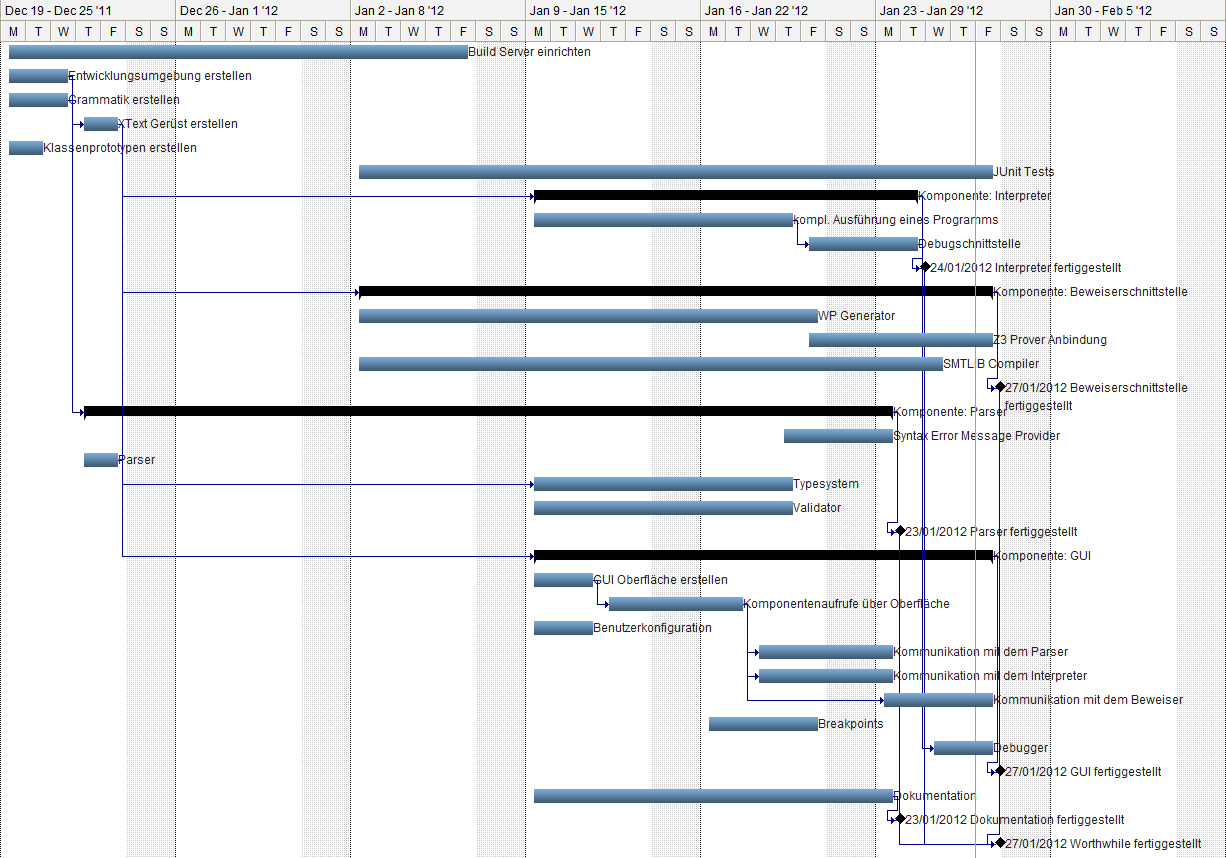
\includegraphics[height=1.2\textheight]{images/gantt_implementierung_diag.png}%
		\caption{Geplanter Ablauf der Implementierungsphase.}%
	\end{figure}%
\end{landscape}
